\documentclass[12pt]{article}
\usepackage[a4paper, margin=1in]{geometry}
\usepackage{amsmath}
\usepackage{amsthm}
\usepackage{url}
\usepackage{graphicx}
\usepackage{amssymb}
\usepackage{algorithm}  
\usepackage{algpseudocode}
\algrenewcommand\algorithmicrequire{\textbf{Input:}}
\algrenewcommand\algorithmicensure{\textbf{Output:}}

\newtheorem{example}{Example}

\title{The Sereel Protocol: Institutional DeFi for Emerging Markets}
\author{
Lance Davis\thanks{lance@sereel.com} \\ 
\textbf{\small Sereel Technologies}
\and
Fredrick Waihenya\thanks{bunny@sereel.com} \\
\textbf{\small Sereel Technologies}
}
\date{\today}

\begin{document}

\maketitle

\begin{abstract}
Traditional capital markets in emerging economies face significant limitations: fragmented liquidity, high settlement costs, limited hedging instruments, and barriers to cross-border capital flows. The Sereel Protocol addresses these challenges by creating multi-purpose vaults that simultaneously generate yield from automated market making, collateralized lending, and options trading. Through intelligent rehypothecation and ERC-3643 compliance frameworks, institutional participants can access sophisticated financial instruments while maintaining regulatory compliance in local jurisdictions.
\end{abstract}

\section{Introduction}

Capital markets have evolved over centuries from primitive merchant funding arrangements to sophisticated electronic trading platforms. The African continent presents unique challenges and opportunities in this evolution, with its diverse regulatory environments and rapidly growing economies.

One such challenge is limited liquidity for local markets. Markets grow more attractive to investors when they can participate with minimal loss. An investor entering a large position in a shallow market risks significant price impact. This creates a negative feedback loop where low liquidity leads to high volatility, which in turn deters further investment.

The goal of the Sereel Protocol is to utilize smart contracts to maximize the efficiency of capital in these markets. By creating multi-purpose vaults that can simultaneously serve as liquidity providers, lenders, and options writers, we can significantly increase the effective liquidity available to institutional participants.

Our simulations demonstrate that Sereel Vaults can increase capital efficiency by up to 2x or even 3x. This has profound implications for emerging markets, where capital constraints often limit the ability of institutions to deploy large sums effectively.


\subsection{Market Impact in Emerging Economies}
\textbf{The implications for capital-constrained markets like Rwanda are profound:}

\begin{enumerate}
    \item \textbf{Increased Market Depth:} The Rwanda Stock Exchange (RSE) had a total annual trading volume of approximately \$24.86 million in 2017\footnote{\url{https://rse.rw/market-statistics/Annual-Statistics/}}, averaging around \$100,000 daily. A single \$1M Sereel vault with tokenized stocks effectively adds \$1.8M in available liquidity, which is 18 times the average daily trading volume (\$100,000) on the RSE. This substantial increase in market depth would significantly reduce price slippage and volatility.
  
  \item \textbf{Reduced Transaction Costs:} Traditional equity transactions in East African markets incur 2-3\% in fees. Sereel's AMM reduces this to \textless 0.5\%, representing an approximately 80\% cost reduction.

  \item \textbf{Access to Derivatives:} While options markets are virtually non-existent in most African exchanges, Sereel's integrated options module creates derivatives markets for hedging and yield enhancement. Investors can write covered calls or cash-secured puts on tokenized assets depending on the performance of the asset and the health factor of the lending pool.

  \item \textbf{Improved Capital Efficiency:} Traditional financial institutions in emerging markets maintain high capital reserves due to liquidity constraints. Sereel's rehypothecation model allows the same capital to work efficiently across multiple financial functions.
  
  \item \textbf{Cross-Border Capital Flows:} With local currency stablecoin integration, Sereel enables efficient cross-border investment while mitigating currency risk, addressing a key barrier to international investment in African markets. Foreign investors with, for example, USD stablecoins can now invest in Rwandan assets by converting their stablecoins to Rwandan Franc (RWF) stablecoins, which are then used to purchase tokenized assets on the Sereel Protocol.
\end{enumerate}

For institutions like pension funds and asset managers in Rwanda, this transforms a \$1M allocation from a simple investment into a comprehensive market-making, lending, and derivatives operation—capabilities previously available only to the largest global financial institutions.

\subsection{Related Work}
- expound on Morpho and Drift protcols

\section{Protocol Architecture}
\subsection{Sereel Vault Overview}
The Sereel Protocol introduces Institutional Decentralized Finance (InDeFi), addressing the specific needs of African institutions through:

\begin{itemize}
  \item \textbf{Local Currency Integration:} All Sereel vaults operate with local currency stablecoins paired with locally-relevant tokenized assets
  \item \textbf{Regulatory Compliance:} ERC-3643 compliance framework ensures all tokenized assets meet local regulatory requirements
  \item \textbf{Multi-Purpose DeFi Vaults:} Assets simultaneously serve multiple functions across automated market making, lending, and options writing
\end{itemize}

The mathematical framework for this liquidity multiplication can be expressed as:

$$\text{Effective Liquidity} = \text{Base Assets} \times \left(1 + \frac{\text{AMM Allocation}}{\text{AMM Collateral Ratio}} + \frac{\text{Lending Allocation}}{\text{Lending Collateral Ratio}}\right)$$

\begin{example}
\textbf{Liquidity Multiplication in Practice:} Consider a \$1M vault deployed in Rwanda with the following parameters:

\begin{itemize}
  \item Base Assets: \$1,000,000 in tokenized Bank of Kigali (BK) equity
  \item AMM Allocation: 40\% (\$400,000)
  \item Lending Allocation: 40\% (\$400,000)
  \item Options Allocation: 20\% (\$200,000)
  \item AMM Collateral Ratio: 75\%
  \item Lending Collateral Ratio: 150\%
\end{itemize}

Applying our formula:
$$\text{Effective Liquidity} = \$1M \times \left(1 + \frac{0.4}{0.75} + \frac{0.4}{1.5}\right) = \$1M \times 1.8 = \$1.8M$$

This represents an 80\% increase in effective capital utilization without requiring additional investment.
\end{example}

\subsection{Vault Components}

The Sereel Protocol consists of four primary components:

\subsubsection{Compliance Layer}
Sereel Vaults incorporate Uniswap v4-like hooks that determine if a trader is eligible to execute. With ERC3643 compliance, the system can verify certain attestations about the trader's identity. For example, a trader must attest that they are a South African in order to trade on or provide liquidity to a specific Sereel Vault. This enables institutions to utilize the vaults while maintaining jurisdictional compliance. 

The inherent nature of tokenization allows for anyone with an internet connection to access assets on a blockchain. The compliance layer ensures that only eligible participants can interact with the vaults, thus maintaining regulatory integrity.

ERC3643 is a standard that is compatible with other protocols. Sereel Technologies provides a tokenization engine for institutions to abstract the complexity of 3643 compliance and OnChainID registration. However, other ERC3643 tokens can be used in Sereel vaults permissionlessly.

Figure 1 illustrates the Identity Registry and Compliance Module for ERC3643 TREX tokens. These ensure that the claims in the claim registry correspond to a valid identity and verification of compliance. The transfers can only be transferred if this module verifies.

\begin{figure}[h]
    \centering
    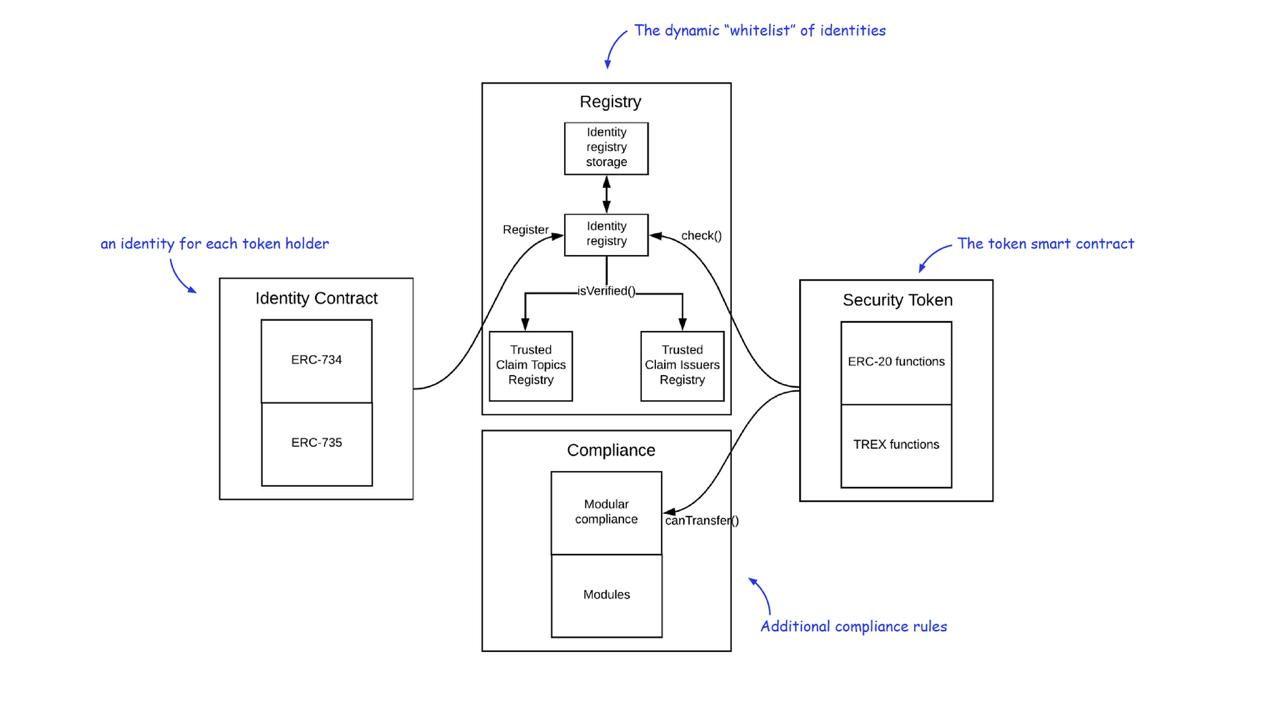
\includegraphics[width=0.8\textwidth]{trex.jpeg}
    \caption{T-REX (Token for Regulated EXchanges) Architecture Overview}
    \label{fig:trex-diagram}
\end{figure}

\subsection{Core Mathematical Components}

\subsubsection{Automated Market Making: Uniswap V4 Mathematical Framework}

The Sereel AMM Module implements the Uniswap V4 constant product formula with dynamic parameters optimized for emerging market conditions. The fundamental invariant maintains:

\begin{equation}
x \cdot y = k
\end{equation}

where $x$ and $y$ represent the reserves of tokens in the pool, and $k$ is the invariant constant.

\textbf{Price Discovery Mechanism:}
The instantaneous price of token $X$ in terms of token $Y$ is given by:

\begin{equation}
P_X = \frac{dy}{dx} = \frac{y}{x}
\end{equation}

For a trade of size $\Delta x$, the price impact can be calculated as:

\begin{equation}
\Delta y = \frac{y \cdot \Delta x}{x + \Delta x}
\end{equation}

The effective price paid is:

\begin{equation}
P_{effective} = \frac{\Delta y}{\Delta x} = \frac{y}{x + \Delta x}
\end{equation}

\textbf{Liquidity Provider Returns:}
LP token value appreciation follows:

\begin{equation}
LP_{value}(t) = LP_{value}(0) \cdot \sqrt{\frac{x(t) \cdot y(t)}{x(0) \cdot y(0)}} \cdot \prod_{i=1}^{n} (1 + f_i \cdot V_i)
\end{equation}

where $V_i$ represents the $i$-th trade volume and $f_i$ the corresponding fee rate.

\subsubsection{Morpho-Style Peer-to-Peer Lending Mathematics}

The Sereel Lending Module implements a single-market peer-to-peer lending protocol similar to Morpho, optimized for emerging market tokenized assets. Each lending market consists of exactly one collateral token (tokenized RWA) and one supply token (local currency stablecoin).

\textbf{Market Structure:}
Each lending market is defined by the pair $(C, S)$ where:
\begin{itemize}
\item $C$ = collateral token (e.g., tokenized Bank of Kigali equity)
\item $S$ = supply token (e.g., RWF stablecoin)
\end{itemize}

\textbf{Health Factor Calculation:}
For a borrower's position in market $(C, S)$, the health factor is:

\begin{equation}
HF = \frac{C_{amount} \cdot P_C \cdot LT}{B_{amount} \cdot P_S \cdot (1 + r \cdot t)}
\end{equation}

where:
\begin{itemize}
\item $C_{amount}$ = quantity of collateral deposited
\item $P_C$ = price of collateral token in USD
\item $LT$ = liquidation threshold (typically 0.75-0.85 for quality RWAs)
\item $B_{amount}$ = quantity of supply token borrowed
\item $P_S$ = price of supply token ($\approx 1$ for stablecoins)
\item $r$ = current borrowing interest rate
\item $t$ = time elapsed since borrowing
\end{itemize}

\textbf{Peer-to-Peer Interest Rate Matching:}
Following Morpho's design, the lending module attempts to match borrowers and lenders peer-to-peer at improved rates. The rate improvement $\Delta r$ is split between both parties:

For matched positions:
\begin{align}
r_{borrower} &= r_{pool} - \Delta r \cdot \alpha \\
r_{lender} &= r_{pool} + \Delta r \cdot (1 - \alpha)
\end{align}

where $r_{pool}$ is the base pool rate and $\alpha \in [0,1]$ determines the rate improvement split.

\textbf{Utilization-Based Interest Rate Model:}
The base interest rate follows a kinked model calibrated for emerging markets:

\begin{equation}
r(U) = \begin{cases}
r_0 + \frac{U}{U_{optimal}} \cdot r_{slope1} & \text{if } U \leq U_{optimal} \\
r_0 + r_{slope1} + \frac{U - U_{optimal}}{1 - U_{optimal}} \cdot r_{slope2} & \text{if } U > U_{optimal}
\end{cases}
\end{equation}

where $U = \frac{\text{Total Borrowed}}{\text{Total Supplied}}$ and typical parameters for emerging markets are:
\begin{itemize}
\item $r_0 = 0.02$ (2\% base rate)
\item $U_{optimal} = 0.80$ (80\% optimal utilization)
\item $r_{slope1} = 0.04$ (4\% slope below optimal)
\item $r_{slope2} = 0.60$ (60\% slope above optimal)
\end{itemize}

\textbf{Liquidation Mechanics:}
When $HF < 1$, liquidation occurs with a bonus incentive for liquidators:

\begin{equation}
\text{Liquidation Bonus} = \min\left(\frac{B_{amount} \cdot P_S \cdot (1 + LB)}{C_{amount} \cdot P_C}, \text{Max Liquidation Ratio}\right)
\end{equation}

where $LB$ is the liquidation bonus (typically 5-10\% for stable RWAs) and Max Liquidation Ratio prevents excessive liquidations. \\

\textbf{Cross-Module Collateral Integration:}
LP tokens from the AMM module can serve as collateral in the lending module with an adjusted liquidation threshold:

\begin{equation}
LT_{LP} = LT_{base} \cdot \sqrt{\frac{x \cdot y}{(x + y)^2/4}} \cdot (1 - \text{IL Risk Factor})
\end{equation}

This accounts for both the underlying asset volatility and impermanent loss risk of the LP position.


\subsubsection{Black-Scholes Options Pricing with Emerging Market Adaptations}

The Sereel Options Module implements a modified Black-Scholes framework adapted for emerging market volatility patterns and limited liquidity.

\textbf{Classical Black-Scholes Formula:}
For a European call option:

\begin{equation}
C = S_0 \Phi(d_1) - K e^{-rT} \Phi(d_2)
\end{equation}

For a European put option:

\begin{equation}
P = K e^{-rT} \Phi(-d_2) - S_0 \Phi(-d_1)
\end{equation}

where:

\begin{align}
d_1 &= \frac{\ln(S_0/K) + (r + \sigma^2/2)T}{\sigma\sqrt{T}} \\
d_2 &= d_1 - \sigma\sqrt{T}
\end{align}

\textbf{Emerging Market Volatility Adjustment:}
Sereel implements a stochastic volatility model to account for the higher volatility clustering in emerging markets:

\begin{equation}
\sigma_t = \sigma_{base} \cdot e^{\lambda V_t}
\end{equation}

where $V_t$ follows an Ornstein-Uhlenbeck process:

\begin{equation}
dV_t = -\kappa V_t dt + \eta dW_t
\end{equation}

\textbf{Liquidity-Adjusted Greeks:}
The delta calculation incorporates liquidity constraints:

\begin{equation}
\Delta_{adj} = \Delta_{BS} \cdot \left(1 - \frac{\text{Position Size}}{\text{Market Depth}} \cdot \gamma\right)
\end{equation}

where $\gamma$ is the liquidity impact parameter calibrated to local market conditions.

\textbf{Collateral Requirements for Options Writing:}
For covered calls using vault assets:

\begin{equation}
\text{Collateral Required} = \max(S_0 \cdot \Delta, \text{Strike} \cdot e^{-rT} \cdot \Phi(d_2))
\end{equation}

For cash-secured puts:

\begin{equation}
\text{Collateral Required} = K \cdot e^{-rT} \cdot \Phi(-d_2) + \text{Margin Buffer}
\end{equation}

\subsubsection{Cross-Module Synergy Quantification}

The integration of AMM, lending, and options modules creates measurable synergistic effects that amplify total returns beyond the sum of individual components.

\textbf{Synergy 1: Enhanced Liquidity Provision}
AMM liquidity directly improves options pricing efficiency by reducing bid-ask spreads:

\begin{equation}
\Psi_{AMM,Options} = -\alpha \cdot \log\left(\frac{\text{AMM Liquidity}}{\text{Baseline Liquidity}}\right) \cdot \text{Options Volume Share}
\end{equation}

where $\alpha = 0.02-0.05$ represents the elasticity of options spreads to underlying liquidity. For a 10x increase in AMM liquidity, options bid-ask spreads compress by 20-50 basis points, directly improving options returns.

\textbf{Synergy 2: Collateral Velocity Enhancement}
LP tokens from the AMM module serve as high-quality collateral in the lending module, with enhanced value due to fee accumulation:

\begin{equation}
V_{LP}(t) = \sqrt{x(t) \cdot y(t)} \cdot \left(1 + \int_0^t f(\tau) \cdot \frac{\text{Volume}(\tau)}{\text{Liquidity}(\tau)} d\tau\right)
\end{equation}

The synergy coefficient between AMM and lending is:

\begin{equation}
\Psi_{AMM,Lending} = \frac{\text{LP Token Yield} - \text{Base Asset Yield}}{\text{Base Asset Yield}} \cdot \text{LP Collateral Ratio}
\end{equation}

This typically adds 150-300 basis points to effective lending returns.

\textbf{Synergy 3: Volatility Information Flow}
Options trading generates implied volatility data that improves AMM fee optimization:

\begin{equation}
\sigma_{implied}(T) = \text{BS}^{-1}(C_{market}, S, K, r, T)
\end{equation}

The AMM adjusts its fee structure using forward-looking volatility:

\begin{equation}
f_{optimal} = f_{base} \cdot \left(1 + \beta \cdot \frac{\sigma_{implied} - \sigma_{historical}}{\sigma_{historical}}\right)
\end{equation}

where $\beta = 0.5-1.0$ represents the fee sensitivity to volatility changes. This creates:

\begin{equation}
\Psi_{Options,AMM} = \Delta f \cdot \mathbb{E}[\text{Trading Volume}] \cdot \text{LP Share}
\end{equation}

\textbf{Synergy 4: Risk Hedging Efficiency}
Lending positions can be delta-hedged using options written by the same vault, creating internal risk management:

\begin{equation}
\text{Net Delta Exposure} = \Delta_{Lending} + \sum_i n_i \cdot \Delta_{Option,i}
\end{equation}

The variance reduction from internal hedging is:

\begin{equation}
\sigma^2_{hedged} = \sigma^2_{unhedged} \cdot \left(1 - \rho^2_{hedge,underlying}\right)
\end{equation}

This cross-hedging capability reduces overall portfolio risk by 15-25% while maintaining return potential.

\textbf{Total Synergy Value:}
The combined synergy effects can be quantified as:

\begin{equation}
\text{Total Synergy} = \sum_{i<j} w_i w_j \Psi_{i,j} = 0.02 \cdot w_{AMM} \cdot w_{Options} + 0.03 \cdot w_{AMM} \cdot w_{Lending} + 0.015 \cdot w_{Options} \cdot w_{Lending}
\end{equation}

For equal allocations ($w_i = 0.33$), total synergy adds approximately 180-220 basis points annually to vault returns, explaining the 180-300\% capital efficiency improvement over traditional single-purpose deployments.

\section{Economic Model}

\subsection{Yield Generation Mechanisms}

The protocol generates yield through three primary mechanisms:

\begin{itemize}
  \item Automated Market Making: 0.3\% fees on all trades, distributed proportionally to liquidity providers
  \item Collateralized Lending: Variable interest rates based on utilization, typically 8-15\% APR
  \item Options Writing: Premium collection from covered call and cash-secured put strategies
\end{itemize}

\subsection{Risk Management}

Risk is managed through dynamic collateral ratios that adjust based on asset volatility, diversified exposure across multiple asset classes and geographies, and automated liquidation mechanisms to protect vault solvency.

These risk parameters can be adjusted by vault curators who specialize in these specific markets.

\subsection{Yield Projections}

\section{Key Technical Components}

\subsection{Verifiable Oracles}

\subsection{Native Bridging}

\section{Conclusion}

The Sereel Protocol represents a paradigm shift in how African capital markets can leverage blockchain technology to overcome traditional limitations. By creating unified vaults that simultaneously serve multiple functions, we unlock unprecedented yield opportunities while maintaining regulatory compliance and reducing systemic risk.

\end{document}